\section{Устойчивость и медленная динамика}

В предыдущем разделе было показано, как меняется топология спектра Флоке. Теперь рассмотрим, как количественно меняется скорость неустойчивости (показатель Ляпунова \(\lambda\)) и какая геометрическая или динамическая характеристика орбиты за это отвечает.

\subsection{Связь показателя Ляпунова с геометрией}
Как было отмечено ранее, показатель \(\lambda = \ln(\max |\mu|)/T\) монотонно убывает вдоль семейства орбит примерно в 6 раз: от \(\lambda \approx 1.95\) в блоке \textit{canonical} до \(\lambda \approx 0.3\) в блоке \textit{arclength}. 

Первоначально возникает гипотеза о том, что эта скорость спада определяется просто периодом \(T\) (то есть \(\lambda \propto T\)). Однако при детальном анализе выясняется, что в плоскости \((T, \lambda)\) траектория семейства образует петли, и монотонной функции \(\lambda(T)\) не существует. 

Оказалось, что гораздо лучшим предиктором является геометрическая характеристика орбиты, названная \textbf{mean\_dev} (среднее отклонение от оси):
\begin{equation}
    \text{mean\_dev} = \frac{1}{T} \int_0^T \sqrt{\sin^2\theta_1 + \sin^2\theta_2} \, dt,
\end{equation}
где \(\theta_1\) и \(\theta_2\) — углы векторов \(\rho_1\) и \(\rho_2\) (расстояний в координатах Якоби) к оси \(X\). По сути, это средняя скорость отклонения тел от коллинеарной конфигурации (оси \(X\)) за период.

На выборке из 208 орбит (41 из \textit{unified} и 167 из \textit{arclength}) была построена линейная регрессия. Корреляция между \(\lambda\) и \textit{mean\_dev} оказалась равной \(r = -0.994\). Если исключить влияние \(T\), частичная корреляция остается \(r = -0.926\). Коэффициент детерминации для модели \(\lambda = a \cdot \text{mean\_dev} + b\) составил \(R^2 = 0.9888\). Это означает, что неустойчивость почти полностью определяется тем, насколько сильно орбита «отклоняется» от оси коллинеарности в среднем за период.

\subsection{Опровержение резонанса 5/4}
В ходе исследования возникла изящная гипотеза о том, что семейство орбит в блоке \textit{arclength} захватывается резонансом 5/4. Действительно, отношение периода орбиты к периоду вращения системы \(T / T_{rot}\) имеет медианное значение \(1.2452\), что всего на \(0.4\%\) отличается от \(5/4 = 1.25\). Кроме того, вход в блок \textit{arclength} происходит при \(idx=1593\), где \(T \approx 7.0252\), что почти совпадает с \(5 \pi / (2\Omega) \approx 7.0248\).

Однако эта гипотеза была отвергнута по двум причинам:
\begin{enumerate}
    \item В блоке \textit{arclength} величина \textit{mean\_dev} меняется всего на \(0.016\), а \(T\) — в пределах \(\pm 0.02\). Этот узкий диапазон создает иллюзию «плато» на графике \(T\) от параметра, в то время как на самом деле функция \(T(\text{mean\_dev})\) монотонно возрастает и не имеет полки, характерной для захвата в резонанс.
    \item Отношение \(T/T_{rot} \approx 1.25\) является случайным совпадением, связанным с точкой входа в каталог. Внутри семейства эта величина плавно меняется.
\end{enumerate}
Таким образом, резонанс 5/4 не является динамическим механизмом, удерживающим орбиты в определенной конфигурации (результат проверки показан на рисунке~\ref{fig:resonance_check}).

\begin{figure}[H]
    \centering
    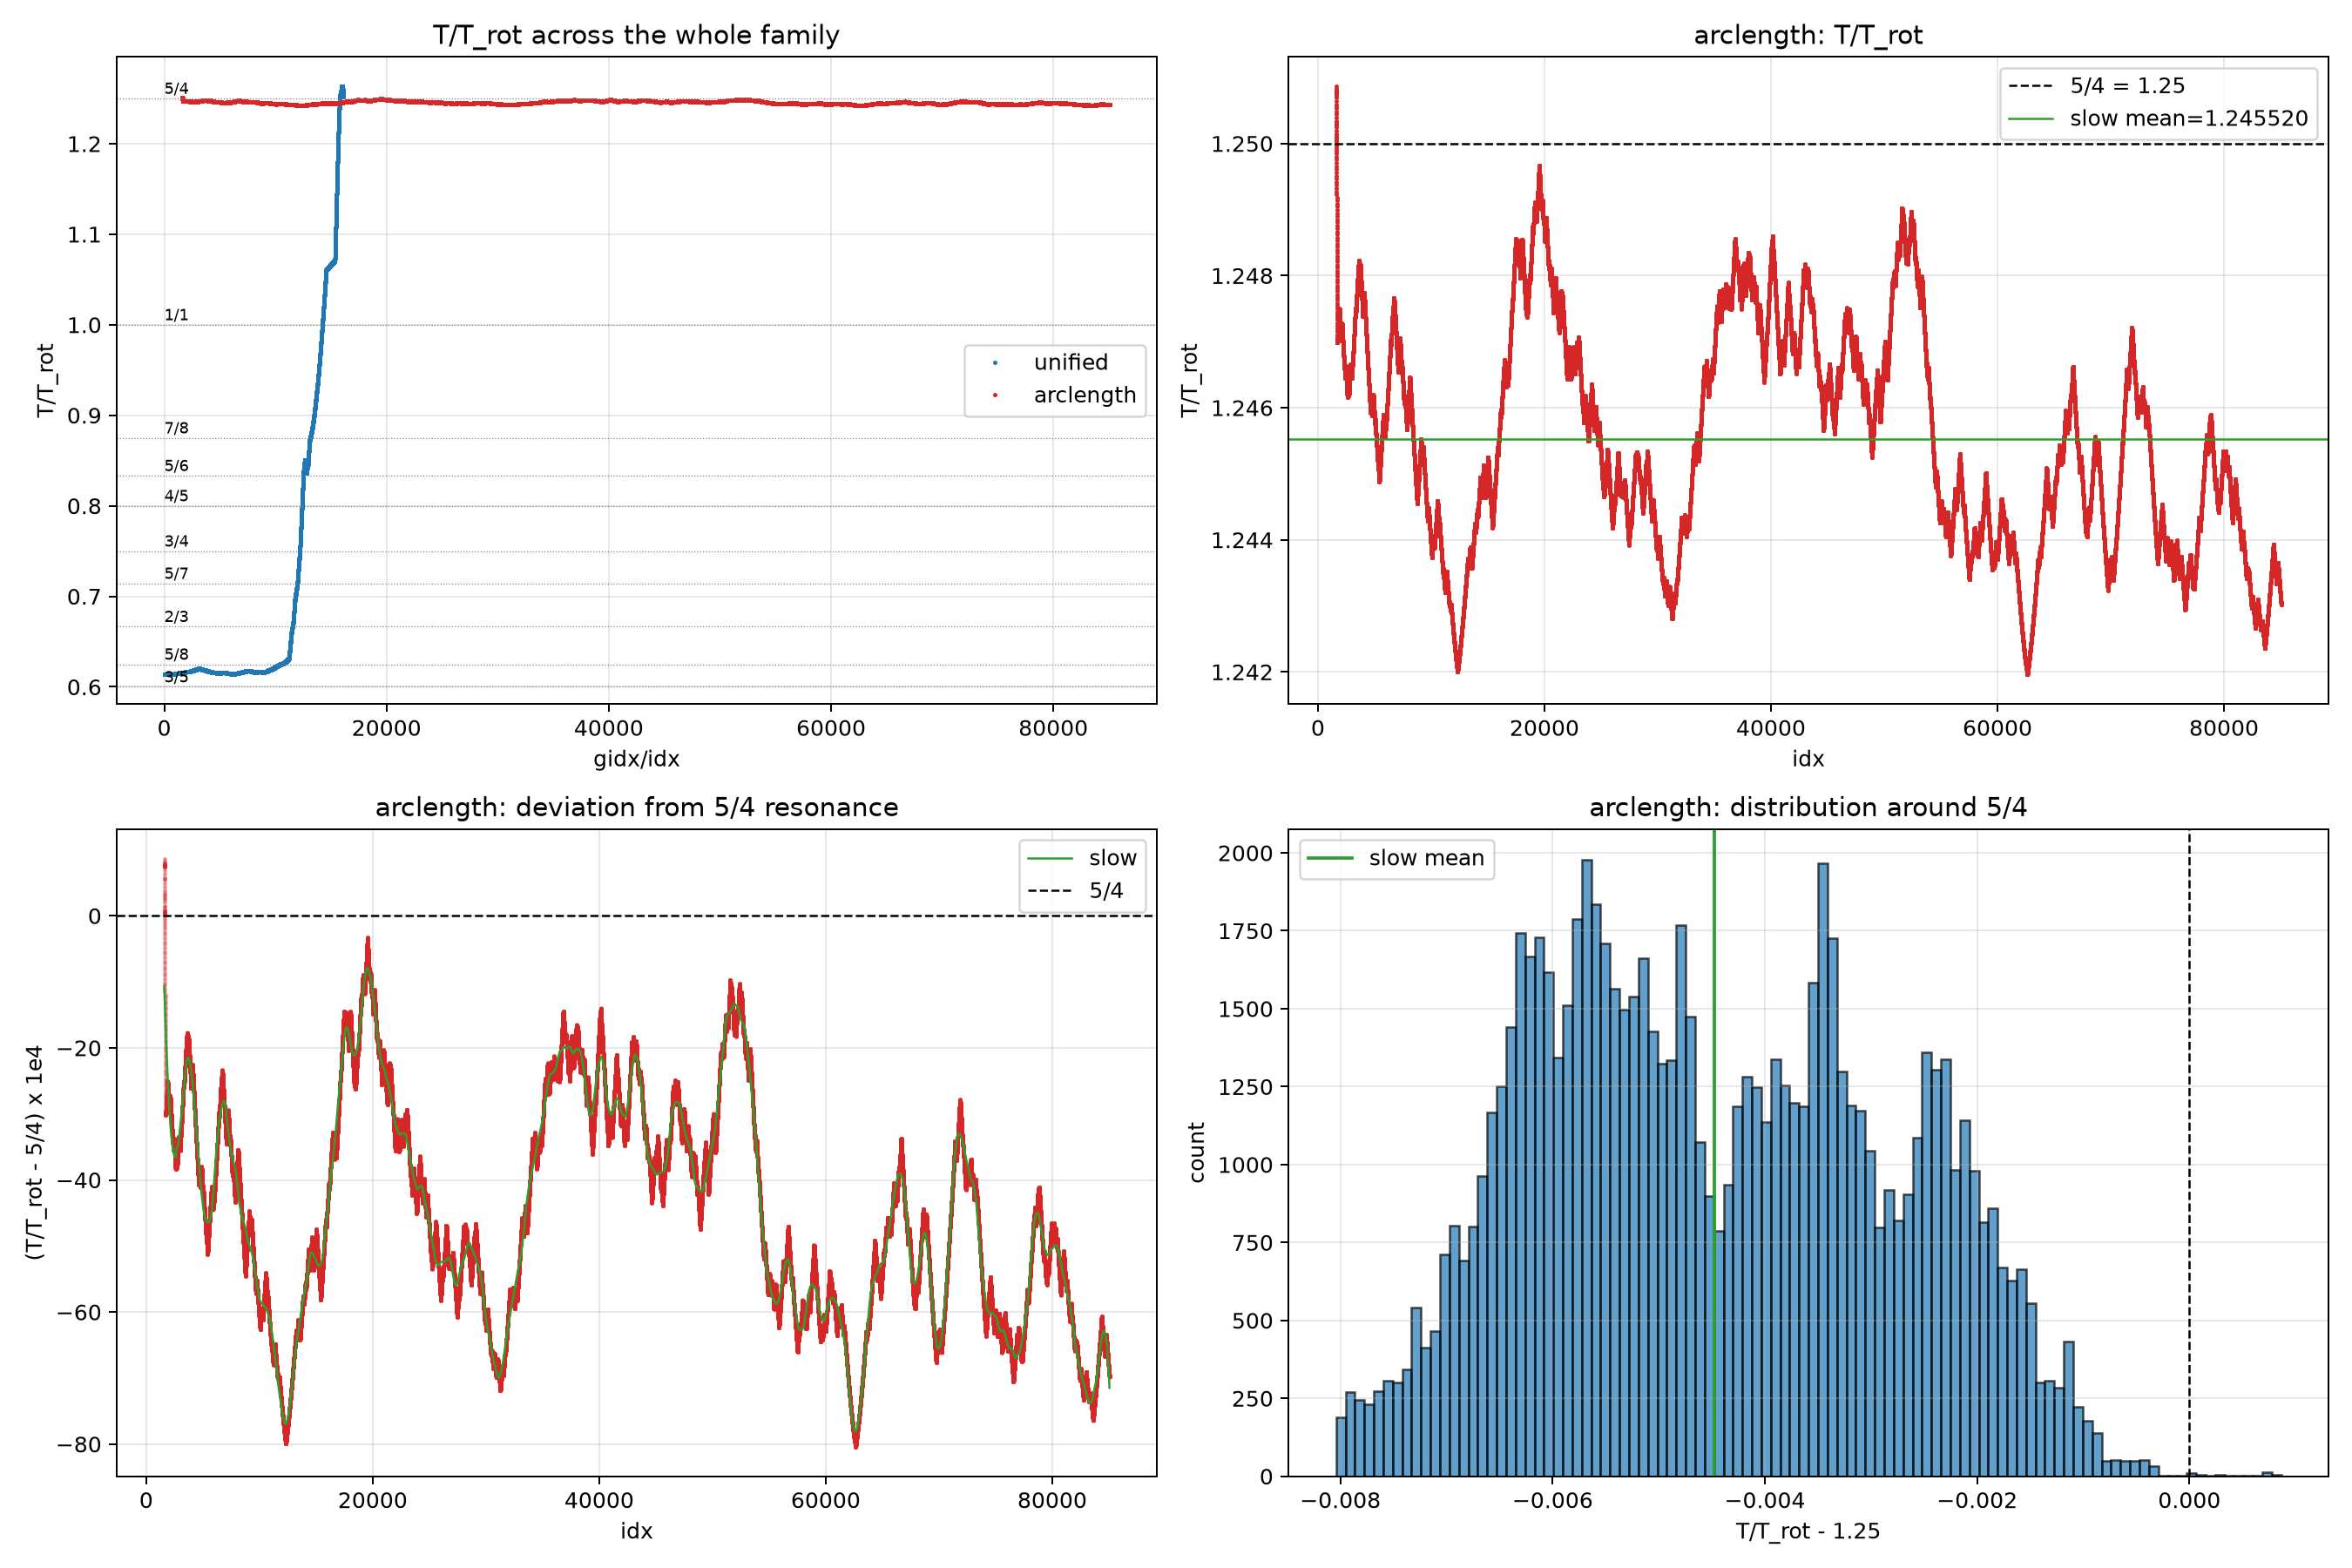
\includegraphics[width=0.75\textwidth]{49_resonance_check.png}
    \caption{Проверка гипотезы о резонансе 5/4. Зависимость периода \(T\) от \textit{mean\_dev} монотонна, «плато» в блоке arclength — следствие узости интервала, а не резонансного захвата.}
    \label{fig:resonance_check}
\end{figure}

\subsection{Широкополосность медленной моды}
Анализ автокорреляционной функции (АCF) и структурной функции орбит (рисунок~\ref{fig:acf}) показал, что так называемая «медленная мода», определяющая форму огибающей орбиты и изменение параметров вдоль семейства, не разлагается на 2–4 четко выраженные гармоники. Она представляет собой широкополосный процесс. Это указывает на сложную нелинейную природу динамики, а не на присутствие одного доминирующего квазипериодического движения.

\begin{figure}[H]
    \centering
    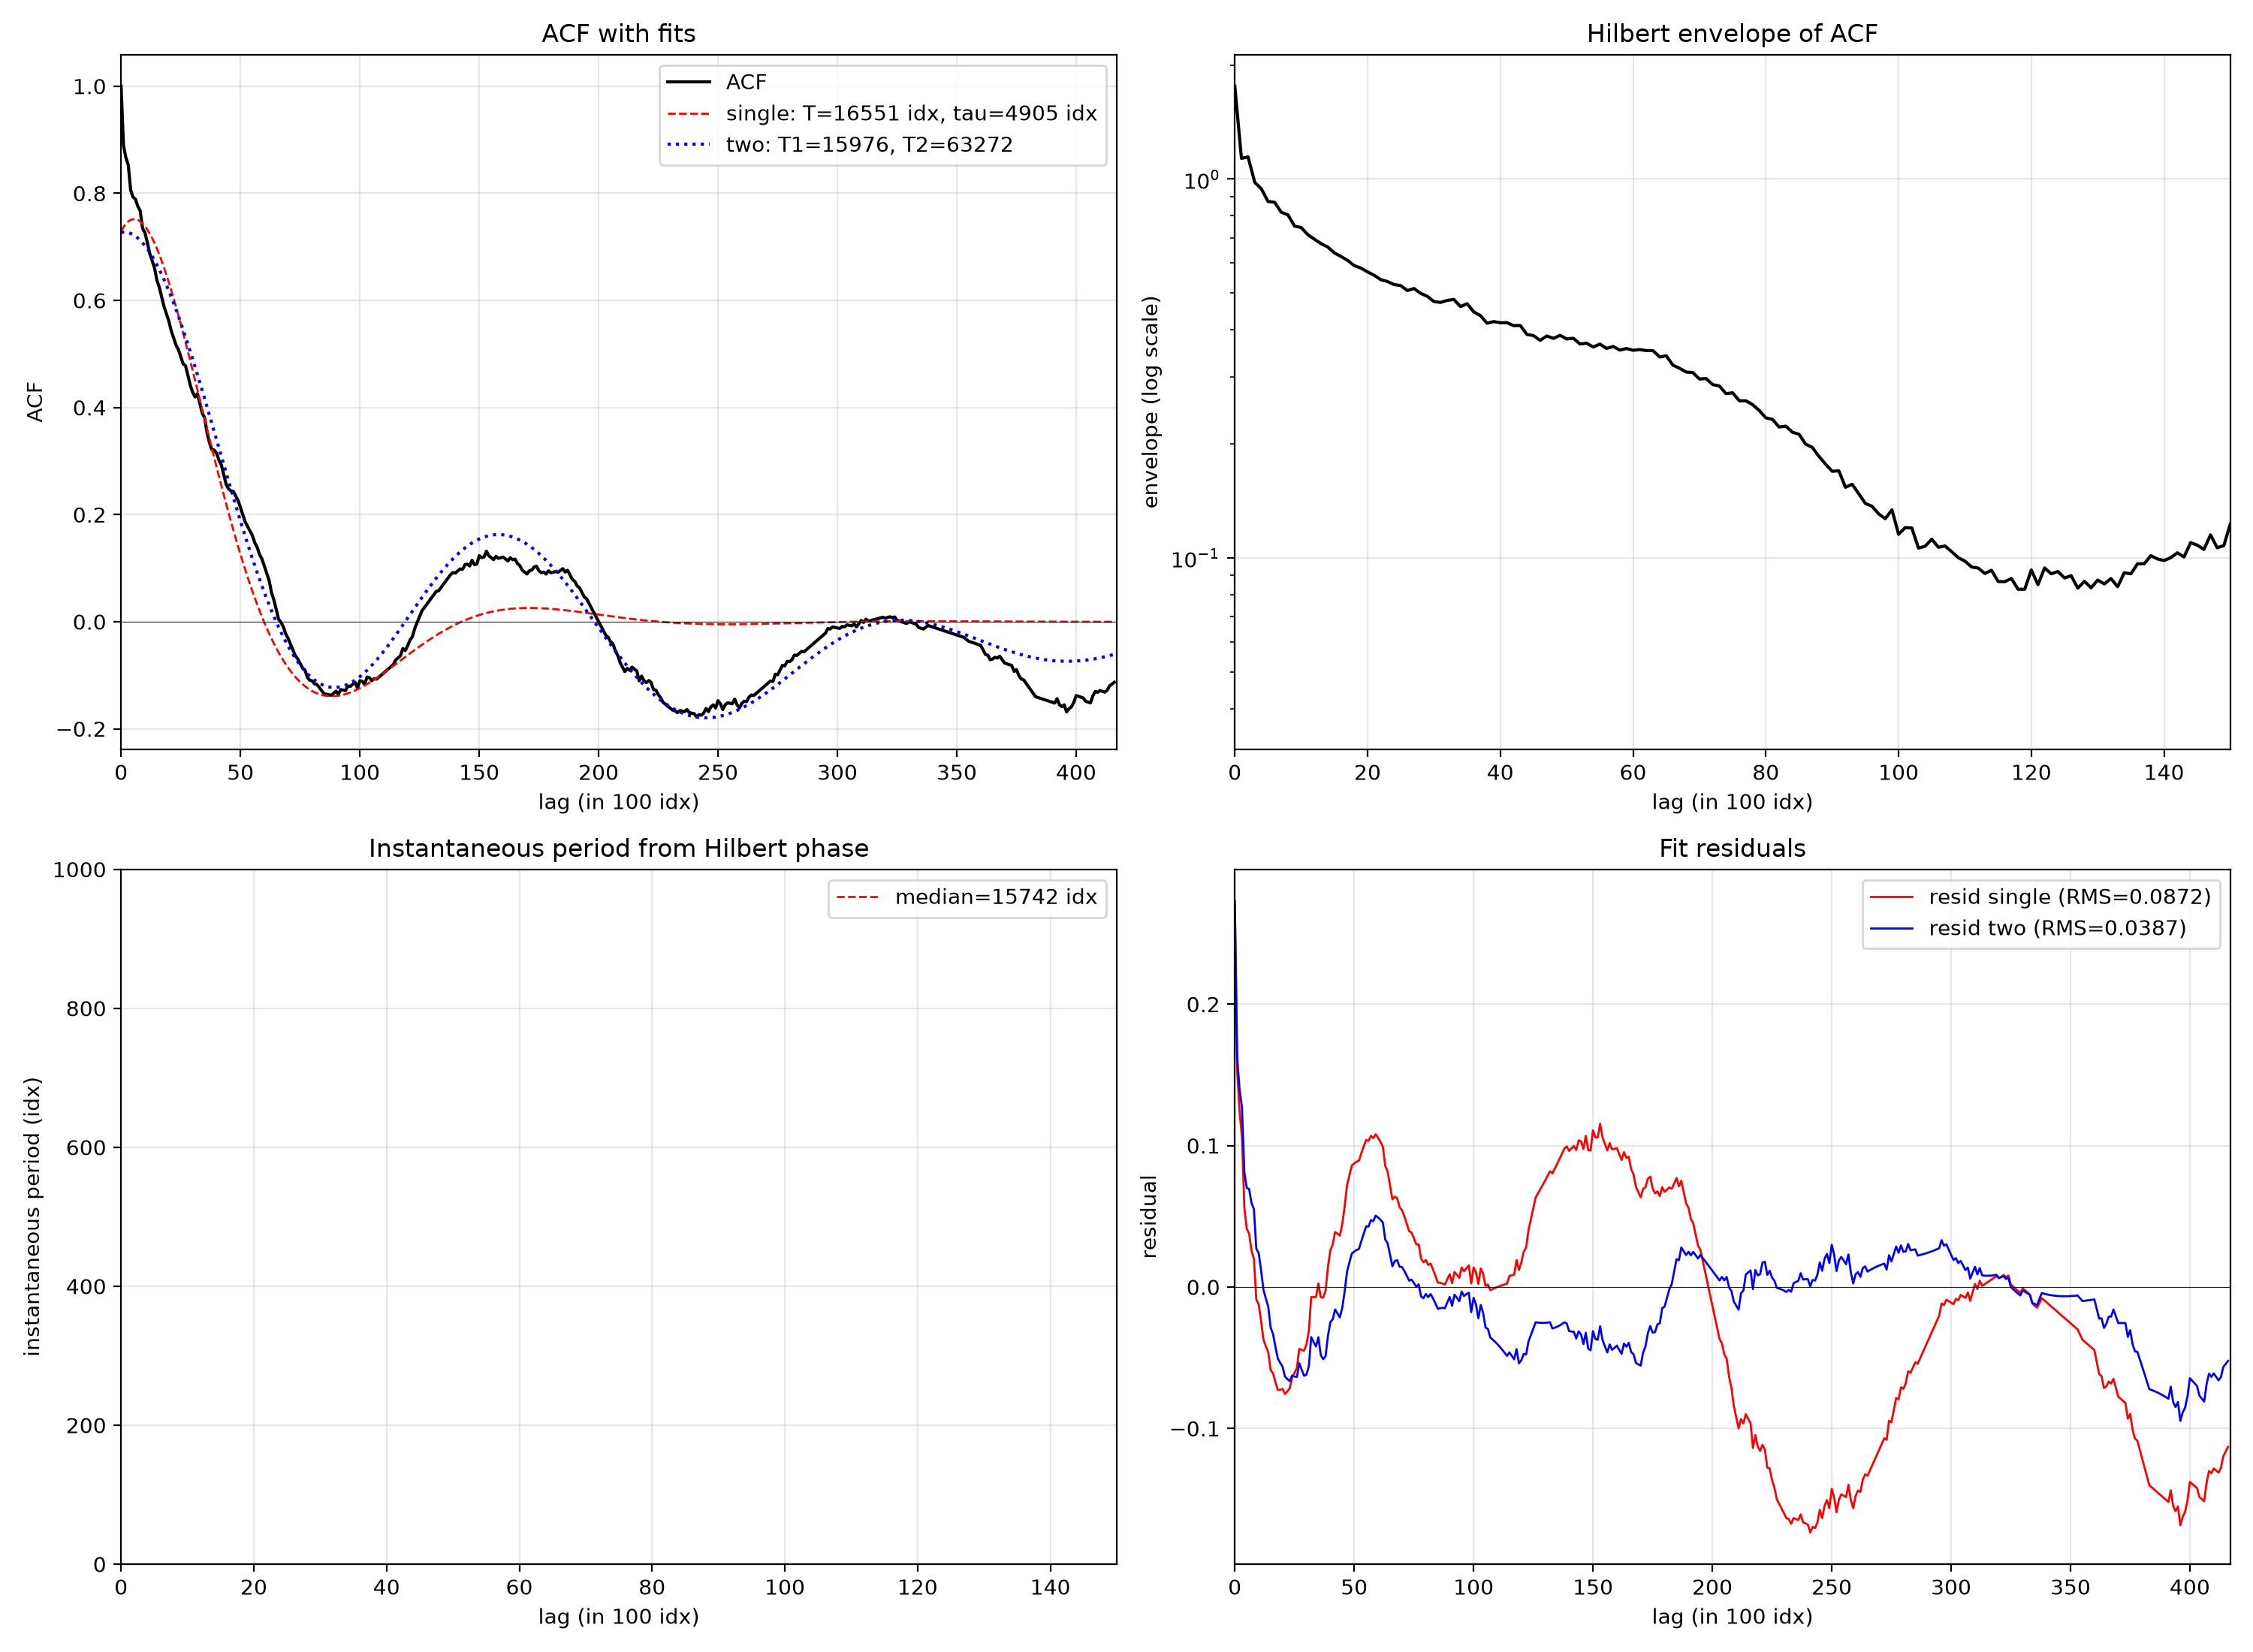
\includegraphics[width=0.75\textwidth]{69_acf_analysis.png}
    \caption{Автокорреляционная функция (ACF), демонстрирующая широкополосный характер медленной динамики вдоль семейства.}
    \label{fig:acf}
\end{figure}

% Общий мастер-плот (по желанию можно вставить здесь или в заключение)
\begin{figure}[H]
    \centering
    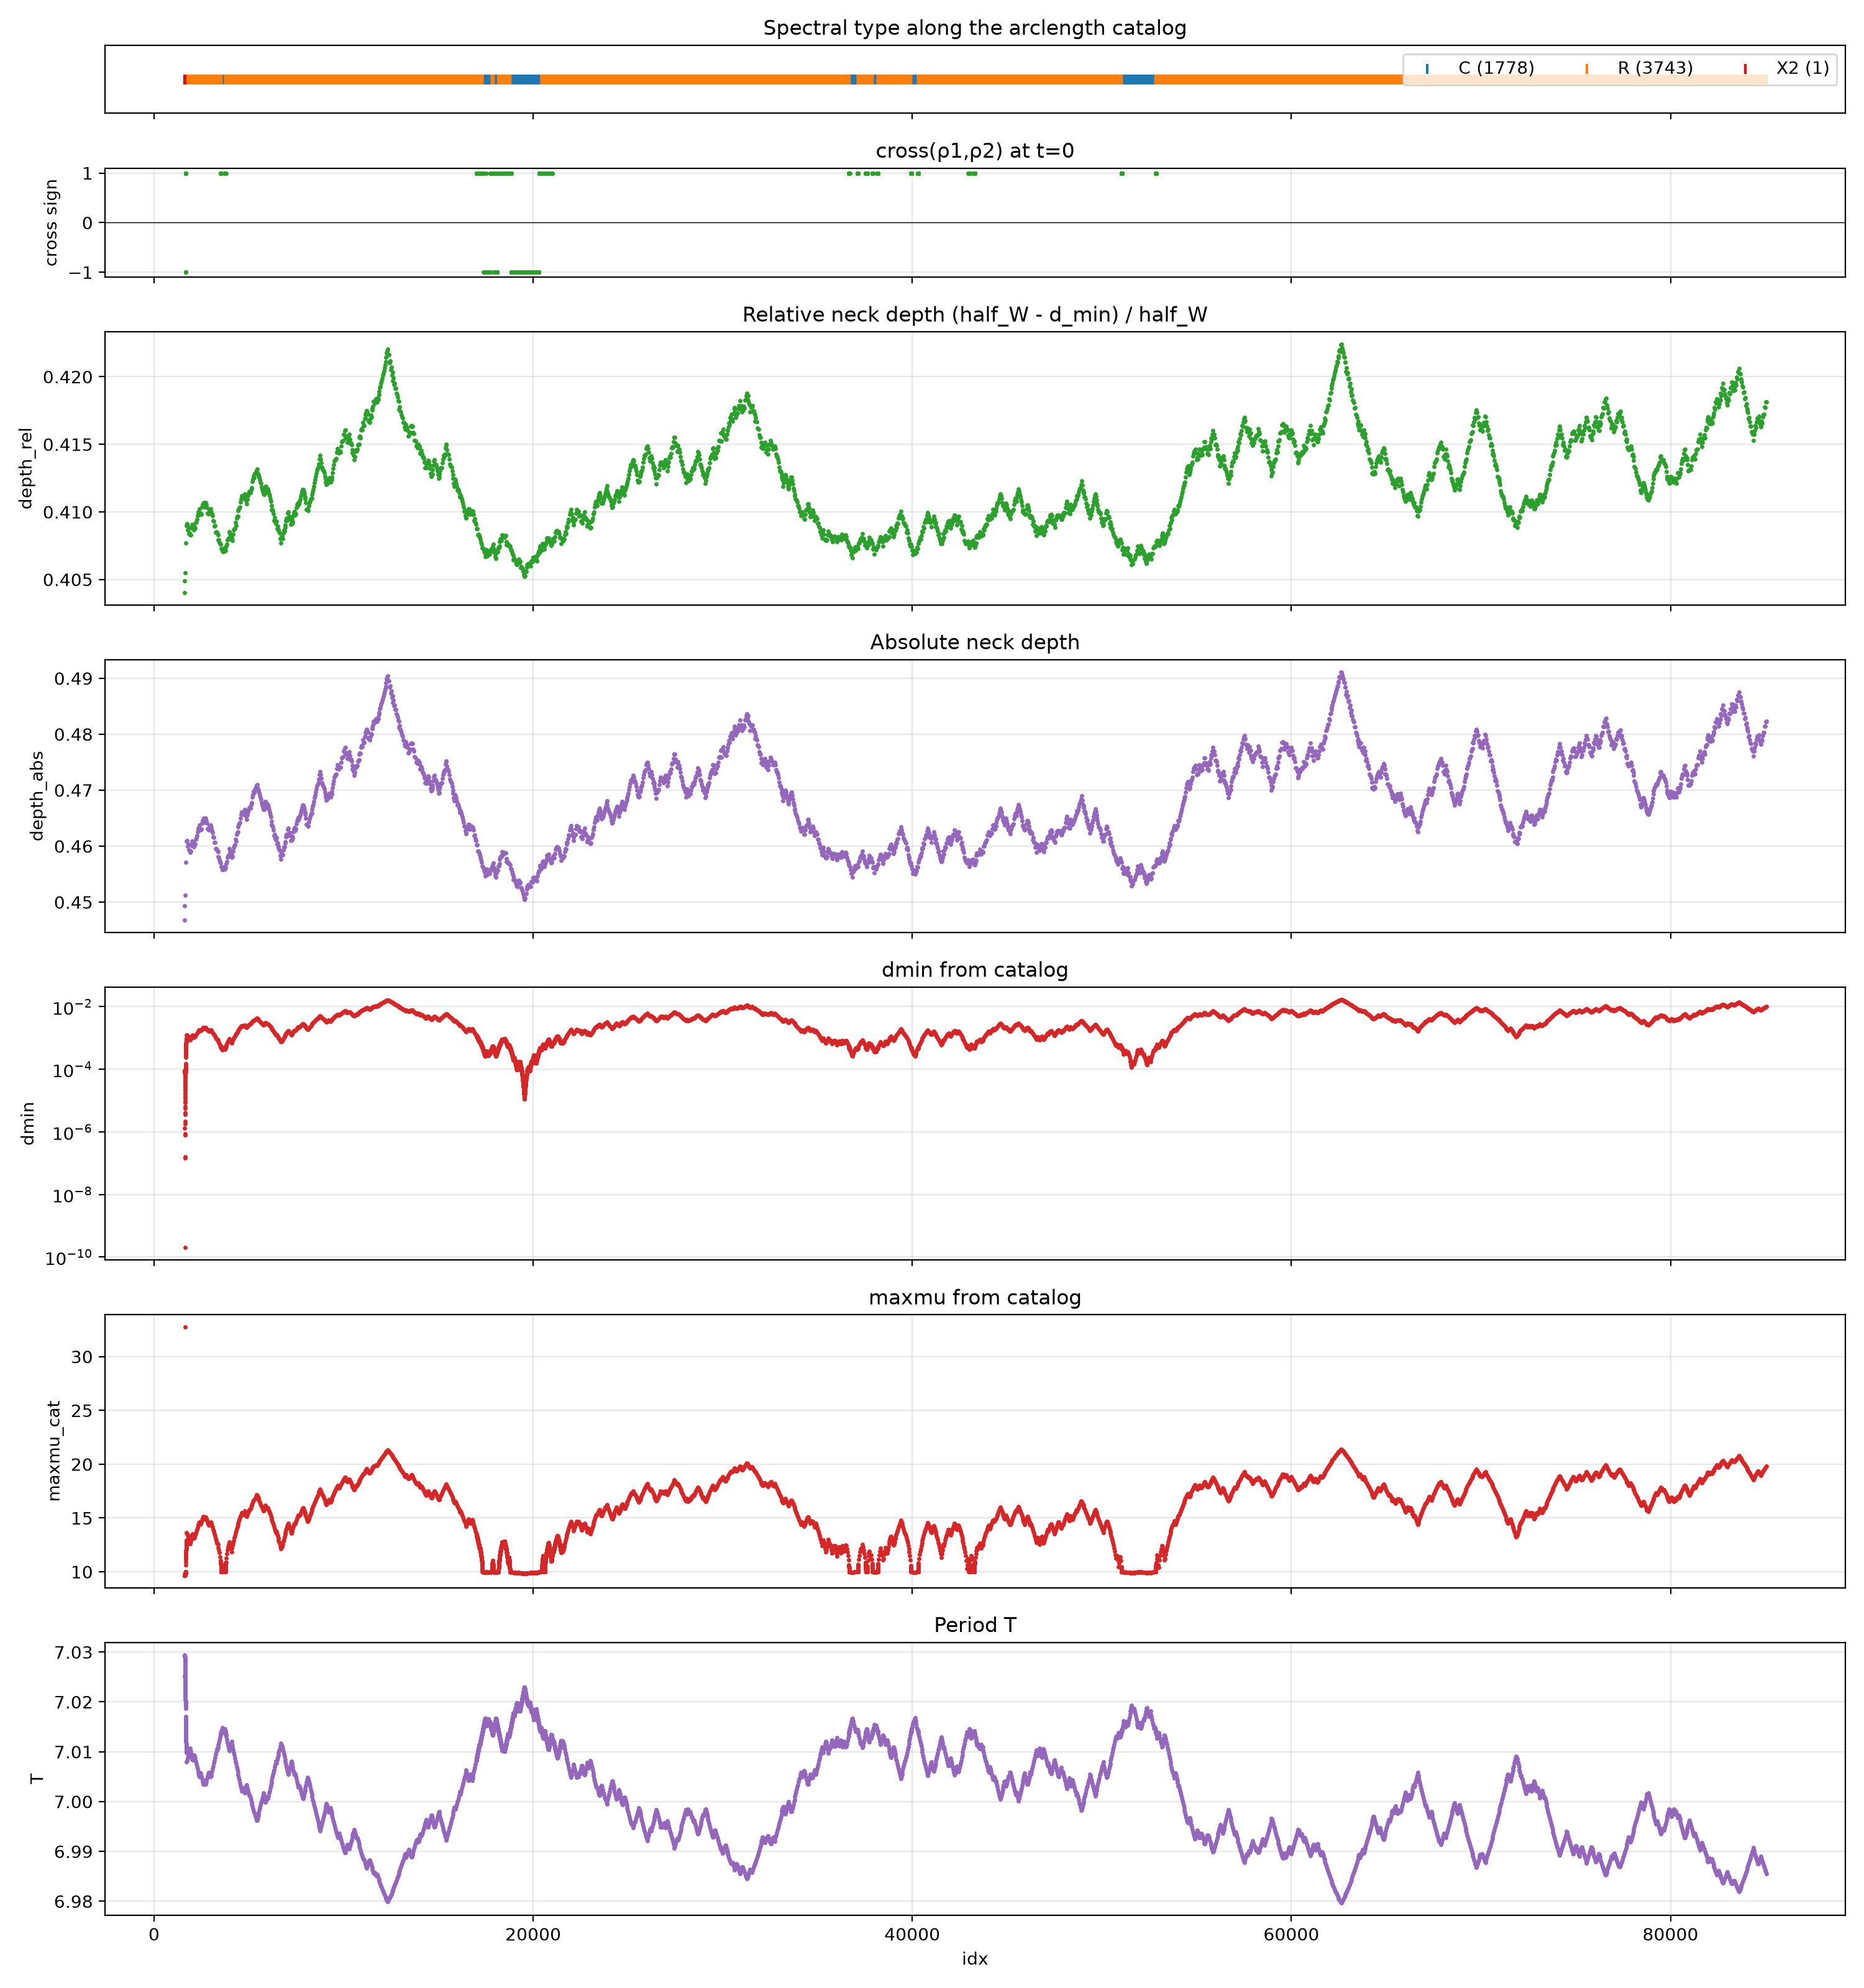
\includegraphics[width=0.95\textwidth]{27_master_plot.png}
    \caption{Общая карта семейства: \(T\), \(\lambda\), \(d_{\min}\), \(\max|\mu|\), глубина ямки и типы спектров.}
    \label{fig:master_plot}
\end{figure}
